%% ****** Start of file template.aps ******%
%%
%%
%%   This file is part of the APS files in the REVTeX 4 distribution.
%%   Version 4.0 of REVTeX, August 2001
%%
%%
%%   Copyright (c) 2001 The American Physical Society.
%%
%%   See the REVTeX 4 README file for restrictions and more information.
%%
%
% This is a template for producing manuscripts for use with REVTEX 4.0
% Copy this file to another name and then work on that file.
% That way, you always have this original template file to use.
%
% Group addresses by affiliation; use superscriptaddress for long
% author lists, or if there are many overlapping affiliations.
% For Phys. Rev. appearance, change preprint to twocolumn.
% Choose pra, prb, prc, prd, pre, prl, prstab, or rmp for journal
%  Add 'draft' option to mark overfull boxes with black boxes
%  Add 'showpacs' option to make PACS codes appear
%  Add 'showkeys' option to make keywords appear
% \documentclass[aps,prl,preprint,groupedaddress]{revtex4}
%\documentclass[aps,prl,preprint,superscriptaddress]{revtex4}
\documentclass[aps,prl,twocolumn,groupedaddress]{revtex4}

\usepackage{amsmath,pdfpages}
%===================================================
% shorthand notations

% LaTeX shortcuts
\newcommand{\la}{\langle}
\newcommand{\ra}{\rangle}

% e.g. & i.e.
\newcommand{\eg}    {{\it e.g.,}\xspace}
\newcommand{\ie}    {{\it i.e.,}\xspace}
\newcommand{\etal}  {{\it et al.}\xspace}

% units
\newcommand{\pe}   {\ensuremath{\,{\rm p.e.}}\xspace}

\newcommand{\pC}   {\ensuremath{\,{\rm pC}}\xspace}

\newcommand{\pers} {\ensuremath{\,{\rm s}^{-1}}\xspace}
\newcommand{\s}    {\ensuremath{\,{\rm s}}\xspace}
\newcommand{\ms}   {\ensuremath{\,{\rm ms}}\xspace}
\newcommand{\us}   {\ensuremath{\,\mu{\rm s}}\xspace}
\newcommand{\ns}   {\ensuremath{\,{\rm ns}}\xspace}
\newcommand{\ps}   {\ensuremath{\,{\rm ps}}\xspace}

\newcommand{\dg}   {\ensuremath{^{\circ}}\xspace}

\newcommand{\Hz}   {\ensuremath{\,{\rm Hz}}\xspace}
\newcommand{\kHz}  {\ensuremath{\,{\rm kHz}}\xspace}
\newcommand{\MHz}  {\ensuremath{\,{\rm MHz}}\xspace}

\newcommand{\fm}   {\ensuremath{\,{\rm fm}}\xspace}
\newcommand{\nm}   {\ensuremath{\,{\rm nm}}\xspace}
\newcommand{\um}   {\ensuremath{\,\mu{\rm m}}\xspace}
\newcommand{\cm}   {\ensuremath{\,{\rm cm}}\xspace}
\newcommand{\m}    {\ensuremath{\,{\rm m}}\xspace}
\newcommand{\km}   {\ensuremath{\,{\rm km}}\xspace}
\newcommand{\cmsq} {\ensuremath{\,{\rm cm}^2}\xspace}
\newcommand{\cmcb} {\ensuremath{\,{\rm cm}^3}\xspace}

\newcommand{\percm}  {\ensuremath{\,/{\rm cm}}\xspace}
\newcommand{\percmsq}{\ensuremath{\,/{\rm cm}^{2}}\xspace}
\newcommand{\percmcb}{\ensuremath{\,/{\rm cm}^{3}}\xspace}
\newcommand{\perm}   {\ensuremath{\,/{\rm m}}\xspace}

\newcommand{\TeV}  {\ensuremath{\mathrm{\,Te\kern -0.1em V}}\xspace}
\newcommand{\GeV}  {\ensuremath{\mathrm{\,Ge\kern -0.1em V}}\xspace}
\newcommand{\MeV}  {\ensuremath{\mathrm{\,Me\kern -0.1em V}}\xspace}
\newcommand{\keV}  {\ensuremath{\mathrm{\,ke\kern -0.1em V}}\xspace}
\newcommand{\eV}   {\ensuremath{\mathrm{\,e\kern -0.1em V}}\xspace}
\newcommand{\GeVc} {\ensuremath{{\mathrm{\,Ge\kern -0.1em V\!/}c}}\xspace}
\newcommand{\MeVc} {\ensuremath{{\mathrm{\,Me\kern -0.1em V\!/}c}}\xspace}
\newcommand{\GeVcc}{\ensuremath{{\mathrm{\,Ge\kern -0.1em V\!/}c^2}}\xspace}
\newcommand{\MeVcc}{\ensuremath{{\mathrm{\,Me\kern -0.1em V\!/}c^2}}\xspace}


% You should use BibTeX and apsrev.bst for references
% Choosing a journal automatically selects the correct APS
% BibTeX style file (bst file), so only uncomment the line
% below if necessary.
%\bibliographystyle{apsrev}

\begin{document}

%\preprint{}

%Title of paper
\title{Anomalous Dispersion at ELANEX, CHERNEAR}

\author{Joel Frederico}
%\email[]{Your e-mail address}
%\homepage[]{Your web page}
%\thanks{}
\altaffiliation{Stanford University}
\affiliation{SLAC Nat'l Accelerator Lab}

%Collaboration name if desired (requires use of superscriptaddress
%option in \documentclass). \noaffiliation is required (may also be
%used with the \author command).
%\collaboration can be followed by \email, \homepage, \thanks as well.
%\collaboration{}
%\noaffiliation

\date{\today}

\begin{abstract}
Dispersion at the lanex screen is anomalous.  The pinch in the butterfly for different quad settings doesn't reflect the calibrated dispersion.  Possible explanations are investigated.  Lessons learned and implemented.
\end{abstract}

\maketitle

\section{Intro}

If you look at the pinch location in the butterfly for different quad settings on Nov.~8, 2013, the pinch is not at the correct energy location.  The dispersion at the lanex screen is expected to be 62~mm, and with a resolution of ~10 $\mu$m/px, the offset of the pinch can be calculated.  This first hinted that the dispersion was wrong.  Rather than go through a calculation of where offsets are to be expected, it is more compelling to calculate the dispersion seen.

There are only 2 independent variables: the calibrated resolution of the camera at ~10 $\mu$/px, which is well-understood per Sebastien; and the matlab function that changed the energy focus at the lanex screen for each step, which I am assured is well-understood per Sebastien and Erik.

The third variable- the pinch location/energy calibration at the lanex screen- is suspect at the moment.  There is one additional assumption made- that the pinch location is actually the location of the energy that is in focus by the quads.  It is possible that this is not true, perhaps through a waist-energy correlation, although I don't think that's the most likely explanation.  One of the best explanations is that there is additional y-dispersion due to tuning/upstream effects.

I will do my best to explore all of these possibilities.

\section{Expected Dispersion}

Per pencil beam/spectrometer magnet scans, the expected dispersion at the near cherenkov wafers is $62\text{mm}$.  The dispersion upstream can be given by:
\begin{align}
	\eta_{lanex} &= \eta_{cher} \frac{\text{distance, spec mag to lanex}}{\text{distance, spec mag to cher}}\\
	&= -\text{62mm} \frac{\text{9.8m}}{\text{10.3m}}\\
	&\approx -\text{57.5mm}
	\label{}
\end{align}

\subsection{Calibrations}

There are several calibrations that go into the measurement of emittance.  Each calibration affects the measurement and must be understood and verified.

\subsubsection{Camera Calibration}

\subsubsection{Dispersion calibration}

\subsubsection{Function to change quads}

\section{Alternate Dispersion Calibrations}

As mentioned previously, the dispersion can be calculated assuming that the quadrupole values are focused correctly and the pinch is representative of the location of the energy in focus.  A rough ROI was selected to track the pinch.  Each ROI was sliced in y in 2-px increments.  Each slice was then fit with a gaussian.  The slices were compiled and fit with a line to recover the dispersion.  The dispersion measured was $\eta_y\approx-23.9\text{mm}$.  There is a difference of roughly $35\text{mm}$ which has to be accounted for.

\begin{figure}
\includegraphics[scale=0.4,page=1]{output.pdf}
\caption{Averaged spot sizes with different energies in focus.}
\end{figure}
\begin{figure}
\includegraphics[scale=0.4]{dispersionfrompinch.eps}
% \caption{Shots are -0.6Gev, -0.4GeV, -0.2GeV, 0GeV, 0.2GeV, 0.4GeV, in the order you'd expect.}
\end{figure}

\section{Comparisons}

\subsection{sYag Energy Spectrum}

The energy content at the yag should be similar to the energy content at the dump table.  If not, could suggest masking.

\subsection{Charge}

If the charge fluctuates at the dump table, not in sync with toros upstream, could also suggest masking.

\subsection{Emittance Measurements}

Quad scan doesn't depend on energy calibration/dispersion, while butterfly measurements do.  I can calculate the dispersion required to make the butterfly measurement match the quad scan.

\subsubsection{Quadrupole Scan}

A traditional quadrupole scan involves refocusing quadrupoles so the transfer matrix $R$ downstream of a point changes in a predictable manner.  As the transfer matrices change, the spot size changes, and can be measured, in this case by the lanex screen:
\begin{align}
	\la x^2 \ra = R_{11}^2 \la x_0^2 \ra + 2R_{11}R_{12} \la x_0 x_0' \ra + R_{12}^2 \la x_0'^2 \ra
	\label{Eq:spot_transfer}
\end{align}
The initial parameters $\la x_0^2 \ra$, $\la x_0 x'_0 \ra$, and $\la x'_0^2 \ra$ can be determined by general linear least squares fitting. These parameters can be converted into emittance, beta, and alpha functions.
\begin{align}
	\epsilon_0 &= \sqrt{\la x_0^2 \ra \la x'_0^2 \ra - \la x_0 x'_0 \ra^2}\\
	\label{Eq:emittance}
	\beta_0 &= \frac{\la x_0^2 \ra}{\epsilon} \\
	% \label{Eq:beta}
	\alpha_0 &= -\frac{\la x_0 x'_0 \ra}{\epsilon}
	% \label{Eq:alpha}
\end{align}

An average image of the 49 shots with the quadrupoles focused at an energy $E=20.35$GeV was taken, and gives a minimum at pixel location of 452px.  The quadrupoles were varied from -0.6GeV to 0.4GeV in 0.2Gev increments, with 49 shots per step.  The 49 images were averaged together, and a strip 2px wide was taken at the location of $E=20.35\text{GeV}$.  The strips were fit with gaussians to recover the variance $\la x^2 \ra$ of the beam.  The initial beam parameters were then recovered per Eq.~\ref{Eq:spot_transfer} and a linear least squares fit.  This gives a measurement of emittance at 153mm-mrad, with Twiss parameters of $\beta=0.136\text{m}$ and $\alpha=-0.194$.
\begin{figure}
	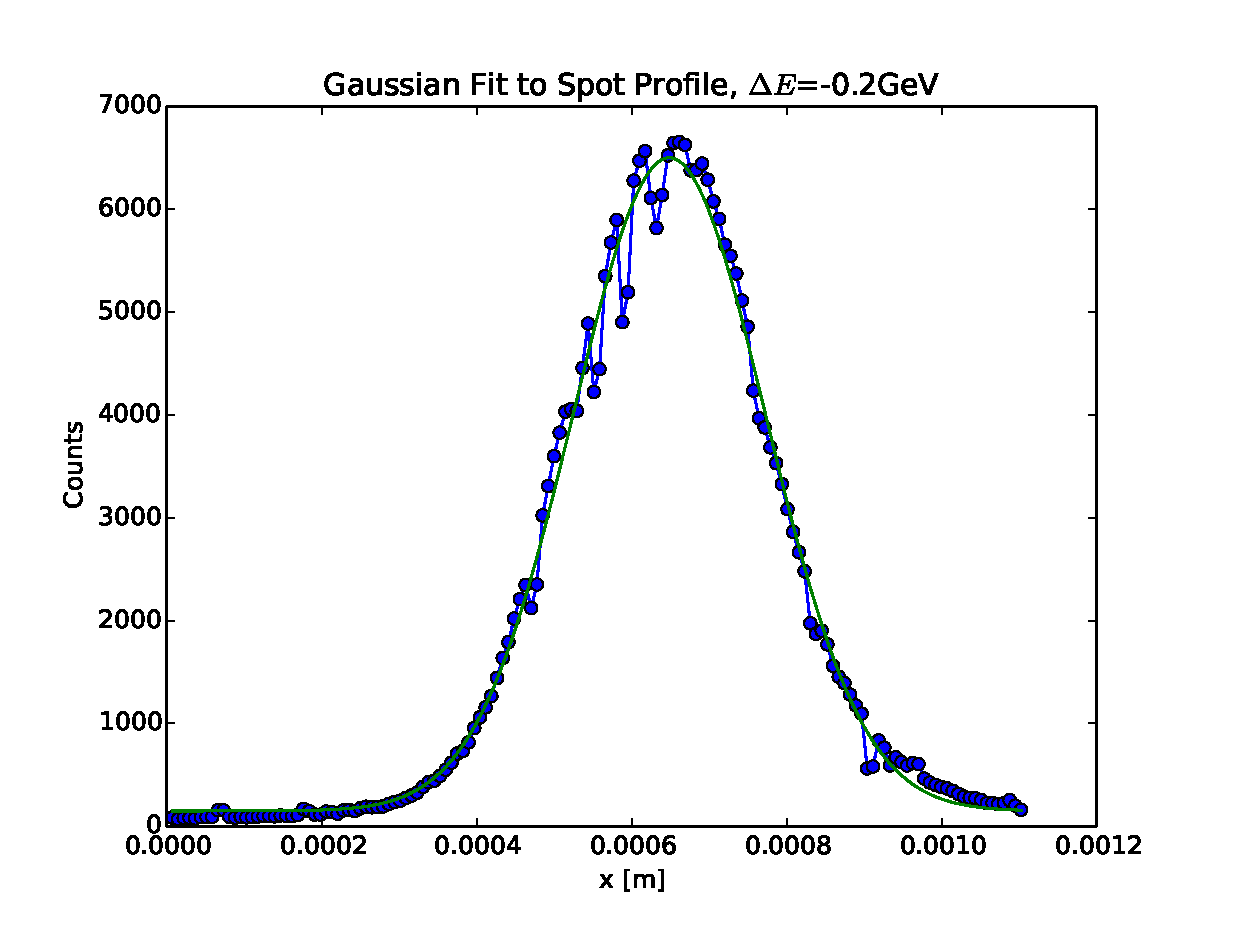
\includegraphics[scale=0.4]{gauss_fit_routine.eps}
	\caption{An example of a gaussian fit to a spot size strip.}
	\label{fig:gaussfit}
\end{figure}
\begin{figure}[]
	\includegraphics[scale=0.4]{quadscanfit.eps}
	\caption{Quadrupole data and its fit.}
	\label{fig:quadscanfit}
\end{figure}

\subsubsection{Butterfly Emittance/Twiss Measurement}

A butterfly emittance and Twiss parameter measurement is a single-shot measurement.  Rather than scanning quadrupoles, different energies are selected away from the in-focus energy at the pinch.  These energies have their own transfer matrices $R_{ij}(E)$.  This requires the ability to transform between energy and location on the lanex screen.

In order to measure the spot size for a given focus/energy, the lanex screen must be calibrated for energy.  The lanex is at a point of high dispersion, and so energies are spread out in $y$ across it.  A calibration consists of determining a reference energy and its location on the screen, determining the dispersion, and determining the resolution in $y$ of the camera system.  Assuming an infinite-energy trajectory is found at $y_\text{mm}=0$, the conversion between pixels and meters can be given by:
\begin{align}
	y_{\text{mm}}&=\text{res}_y \left( y_\text{px} + y_\text{offset} \right)
\end{align}
Given the dispersion at a point $y_c$, the energy for the rest of the lanex can be calibrated.  The dispersion was measured to be $-62\text{mm}$ at the cherenkov air gap, and can be converted to a dispersion measurement at the lanex by scaling the dispersion by the ratio of the distance to the lanex at 9.28m vs. the distance to the cherenkov air gap at 10.33m.  This gives $\eta_{y,lanex}=\eta_{y,cher} \left( 9.28\text{m}/10.33\text{m}  \right) = -55.7\text{mm}$.  The energy at a given point $y$ can be described as
\begin{align}
	y_\text{mm} &= \frac{ e v B l L }{E} \\
	&= \frac{evBlL}{(1+\delta)E_0}
	\label{Eq:e(y)}
\end{align}
where $v\approx c$ is constant, $l$ is the length of the magnet, and $L$ is distance from the magnet to the lanex.  Transverse dispersion is defined as:
\begin{align}
	\eta_y(\delta) &\equiv \frac{d}{d\delta}y(\delta) \\
	&= -\frac{evBlL}{E_0} \frac{1}{\left( 1+\delta \right)^2}
	\label{}
\end{align}
The calibration of dispersion gives $\eta_y(\delta=0)=-\frac{evBlL}{E_0}$. Translating units to pixels gives a final calibration equation of
\begin{align}
	y_\text{px} &= -\frac{1}{\text{res}_y} \frac{\eta_{y,\text{lanex}}}{1+\delta} - y_\text{offset}
	\label{}
\end{align}

With the lanex screen, the location of the pinch in $x$ must be determined in order to calibrate $y_\text{offset}$.  Then
\begin{align}
	y_\text{offset} &= -\frac{\eta_{y,\text{lanex}}}{\text{res}_y} - y_\text{px}
	\label{}
\end{align}



\section{Possible Explanations}

\subsection{Orbit}

If there are steering concerns, changing the quads could move the pinch up and down and imitate dispersion.  This seems unlikely, as the beam as a whole isn't seen to move up and down, just the pinch.  It would have to be combined with some sort of dumpline energy acceptance at the 3\% level, which also seems unlikely.

\subsection{Quad Offsets}

It's also possible there are quad offsets.  This is similar to orbit concerns.

\subsection{Waist-Energy Correlation}

One proposed idea for chromatics is that there could be a slice energy-alpha correlation:
\begin{align}
	\alpha(\delta) &= \alpha_0 + \alpha_0' \delta
	\label{Eq:chromaticalpha}
\end{align}
This probably can't explain things to the $\Delta\eta_y=25$mm level, looking at equations from Sebastien.

\section{Path to ``Proving'' Measurement}

\begin{itemize}
	\item Internally consistent- different measurement methods at the dump table match.
	\item Externally consistent- matches trusted measurements at other locations.
	\item The above issues are shown to not be a problem.
	\item Theory-consistent- measurement value is believable/explainable
	\item Data- In a variety of scenarios (pencil? full-spectrum, different focuses) the measurement works
	\item Present- Present analysis for challenge.
\end{itemize}


% \begin{figure}
% \includegraphics{}%
% \caption{\label{}}
% \end{figure}


% Create the reference section using BibTeX:
% \bibliography{basename of .bib file}

\end{document}
%
% ****** End of file template.aps ******


